% \documentclass[12pt]{article}
\documentclass[12pt]{report}
%\documentclass{report} % 10pt
% Change "article" to "report" to get rid of page number on title page
\usepackage{amsmath,amsfonts,amsthm,amssymb}
\usepackage{setspace}
\usepackage{fancyhdr}
\usepackage{lastpage}
\usepackage{extramarks}
\usepackage{chngpage}
\usepackage{soul}
\usepackage[usenames,dvipsnames]{color}
\usepackage{graphicx,float,wrapfig}
\usepackage{ifthen}
\usepackage{listings}
\usepackage{courier}
%\usepackage[bw,framed,numbered]{mcode}
\usepackage{microtype}
\usepackage{appendix}
\usepackage{hyperref}
\usepackage[all]{hypcap}
\usepackage{url}

% Uncomment this to add line numbers for debugging only.
\usepackage{lineno}
\def\linenumberfont{\normalfont\small\sffamily}
\linenumbers

%\definecolor{MyDarkGreen}{rgb}{0.0,0.4,0.0}

% Needed for changing the font size in \documentclass{} while
% using the fancyhdr package. Else the warning:
% \headheight is too small (12.0pt):Make it at least 14.49998pt.
\setlength{\headheight}{15pt}

% For faster processing, load Matlab syntax for listings
%\lstloadlanguages{Matlab}%
%\lstset{language=Matlab,
%        frame=single,
%        basicstyle=\small\ttfamily,
%        keywordstyle=[1]\color{Blue}\bf,
%        keywordstyle=[2]\color{Purple},
%        keywordstyle=[3]\color{Blue}\underbar,
%        identifierstyle=,
%        commentstyle=\usefont{T1}{pcr}{m}{sl}\color{MyDarkGreen}\small,
%        stringstyle=\color{Purple},
%        showstringspaces=false,
%        tabsize=5,
%        % Put standard MATLAB functions not included in the default
%        % language here
%        morekeywords={xlim,ylim,var,alpha,factorial,poissrnd,normpdf,normcdf},
%        % Put MATLAB function parameters here
%        morekeywords=[2]{on, off, interp},
%        % Put user defined functions here
%        morekeywords=[3]{FindESS},
%        morecomment=[l][\color{Blue}]{...},
%        numbers=left,
%        firstnumber=1,
%        numberstyle=\tiny\color{Blue},
%        stepnumber=0
%        }

% In case you need to adjust margins:
\topmargin=-0.55in
\evensidemargin=0in
\oddsidemargin=0in
\textwidth=6.5in
\textheight=9.25in
\headsep=0.25in

% Homework Specific Information
\newcommand{\hmwkTitle}{Thesis}
\newcommand{\hmwkSubTitle}{Robot Traffic School}
\newcommand{\hmwkDueDate}{June 11, 2010}
\newcommand{\hmwkClass}{MAE}
\newcommand{\hmwkClassTime}{}
\newcommand{\hmwkClassInstructor}{Prof. Bewley}
\newcommand{\hmwkAuthorName}{Thomas Denewiler}
\newcommand{\hmwkAuthorEmail}{tdenewiler@gmail.com}

% Setup the header and footer
\pagestyle{fancy}
\lhead{\hmwkAuthorName}
\chead{\hmwkClass\ (\hmwkClassInstructor) \hmwkTitle}
\rhead{\firstxmark}
\lfoot{\lastxmark}
\cfoot{}
\rfoot{Page\ \thepage\ of\ \protect\pageref{LastPage}}
\renewcommand\headrulewidth{0.4pt}
\renewcommand\footrulewidth{0.4pt}

% Adds a hyperlink to an email address.
\newcommand{\mailto}[2]{\href{mailto:#1}{#2}}

% These commands set the document properties for the PDF output. Needs the hyperref package.
\hypersetup
{
    colorlinks,
    linkcolor={black},
    citecolor={black},
    filecolor={black},
    urlcolor={black},
    pdfauthor={\hmwkAuthorName <\mailto{\hmwkAuthorEmail}{\hmwkAuthorEmail}>},
    pdfsubject={\hmwkClass},
    pdftitle={\hmwkTitle},
    pdfkeywords={UC San Diego, Sensor Networks, Autonomous Underwater Vehicle},
    pdfstartpage={1},
}

% Includes a figure
% The first parameter is the label, which is also the name of the figure
%   with or without the extension (e.g., .eps, .fig, .png, .gif, etc.)
%   IF NO EXTENSION IS GIVEN, LaTeX will look for the most appropriate one.
%   This means that if a DVI (or PS) is being produced, it will look for
%   an eps. If a PDF is being produced, it will look for nearly anything
%   else (gif, jpg, png, et cetera). Because of this, when I generate figures
%   I typically generate an eps and a png to allow me the most flexibility
%   when rendering my document.
% The second parameter is the width of the figure normalized to column width
%   (e.g. 0.5 for half a column, 0.75 for 75% of the column)
% The third parameter is the caption.
\newcommand{\scalefig}[3]{
  \begin{figure}[ht!]
    % Requires \usepackage{graphicx}
    \centering
	\fbox{
	    \includegraphics[width=#2\columnwidth]{#1}
	}
    %%% I think \captionwidth (see above) can go away as long as
    %%% \centering is above
    %\captionwidth{#2\columnwidth}%
    \caption{#3}
    \label{#1}
  \end{figure}}

% Includes a MATLAB script.
% The first parameter is the label, which also is the name of the script
%   without the .m.
% The second parameter is the optional caption.
%\newcommand{\matlabscript}[2]
%  {\begin{itemize}\item[]\lstinputlisting[caption=#2,label=#1]{#1.m}\end{itemize}}

%%%%%%%%%%%%%%%%%%%%%%%%%%%%%%%%%%%%%%%%%%%%%%%%%%%%%%%%%%%%%
% Make title
\title{\vspace{2in}\textmd{\textbf{\hmwkClass:\ \hmwkTitle\ifthenelse{\equal{\hmwkSubTitle}{}}{}{\\\hmwkSubTitle}}}\\\normalsize\vspace{0.1in}\small{Due\ on\ \hmwkDueDate}\\\vspace{0.1in}\large{\textit{\hmwkClassInstructor\ \hmwkClassTime}}\vspace{3in}}
\date{}
\author{\textbf{\hmwkAuthorName}}
%%%%%%%%%%%%%%%%%%%%%%%%%%%%%%%%%%%%%%%%%%%%%%%%%%%%%%%%%%%%%

\begin{document}
\begin{spacing}{1.1}
\maketitle
\thispagestyle{empty}

% Add an empty page after the title page. Looks better when printing double-sided.
\newpage
\thispagestyle{empty}
\mbox{}
\newpage
\pagenumbering{arabic}

% Uncomment the \tableofcontents and \newpage lines to get a Contents page
% Uncomment the \setcounter line as well if you do NOT want subsections
%       listed in Contents
% \setcounter{tocdepth}{1}
\tableofcontents
\clearpage
\listoffigures
\listoftables
\clearpage

%%%%%%%%%%%%%%%
% Introduction.
%%%%%%%%%%%%%%%
\chapter{Introduction}
Robots have been developed to assist humans in tasks that are generally considered dirty, dangerous or boring. Recently robots have found a useful niche as a tool to help Expolosives Ordinance Disposal (EOD) teams to assess and eliminate threats due to improvised explosive devices (IEDs), commonly referred to as roadside bombs, by allowing humans to maintain a safe stand-off distance while investigating a scene. Clearly this falls under the dangerous category. The current method that EOD teams use involves teleoperation of the robot to get from the base to the object of interest. In the process of teleoperating the robot the operator is exposed and vulnerable to other external threats in the area. As technologies mature to provide humans with better tools shortcomings are discovered, such as the vulnerability due to teleoperation, and that opens up avenues for improvement in the development of these tools. For robots one approach to reducing the amount of work humans are required to perform is to give the robots more intelligence via autonomous behaviors using additional sensors, more specialized actuators and software to automate the largest amount of routine tasks as possible.

When adding autonomy to robots nearly all of the tasks can be summarized by the following questions:
\begin{itemize}
\item Where am I?
\item What's around me?
\item Where do I want to go?
\item How do I get there?
\end{itemize}

The initial attempt at adding autonomy to the EOD robots resulted in somewhat erratic driving behavior, especially near obstacles, as the robot trajectory would be very jerky *** needs a better description *** when it changed speed and attempted to make small corrections to its original path to move around the obstacle. In this paper I will look at smoothing out the trajectories taken by the robot by looking for improvements in the state estimation (Where am I?) and controls (How do I get there?) algorithms. For this work I am ignoring actual obstacle detection (What's around me?) and will be using a simple planning algorithm (Where do I want to go?) to simulate obstacles in the robot path which will force the robot to change direction and speed multiple times.

*** Talk more about how this problem is not isolated to any one issue and that state estimation, control and sensor measurements all need to be considered. I need to show later how each piece contributes to making the robot drive better. ***
\clearpage

%%%%%%%%%%%%%
% Background.
%%%%%%%%%%%%%
\chapter{Background}
*** Put in a description of the PackBot, Talon and Urbot along with a description of the algorithms originally used and the results obtained using those algorithms. Talk about JAUS and MOCU a little bit. Discuss more about how the robots are used by EOD. Include that for robots to drive around on their own all they require is an estimate of where they are, a path to follow, a controller to determine the actuator outputs and motor controllers to perform the controller outputs. ***

\section{PackBot}

\section{Talon}

\section{Urbot}

\section{MOCU \& JAUS}

\section{The Duals: Estimation \& Controls}
It is very difficult to simply work on either state estimation or controls individually as there is a large amount of coupling between the two areas. Although the main goal is to make the robots drive more smoothly and that the actuator and motor outputs are ultimately generated by the control system it is still the case that the role of state estimation is equally important. If there exists large meaurement errors, drift or bias in the sensor readings then the robot will not have a very good idea of where it is locted and there will not be a controller that can stabilize the system. *** Talk about observability and controllability. Mention theory that shows link between estimation and control. ***

An example would be when the only sensor available for measurements is an IMU which suffers from drift and bias, where both effects are exagerrated by temperature. There have been situations in which an IMU was in a robot with the motors turned off so that the robot is not moving. However, due to excessive heat in the electronics bos the IMU measurements report that the heading of the robot keeps moving in circles at a rate of $\frac{\pi}{5} rad/s$. With a controller that was known to keep the robot stable when the IMU was working properly started forcing the robot to turn in circles when the motors were turned on even thought the command was to stay in one place. This shows the importance of state estimation on overall robot performance -- it is not enough to only have a good controller.

\clearpage

%%%%%%%%%%%%%%%%%%%
% Related Work.
%%%%%%%%%%%%%%%%%%%
% \section{Related Work}
% \clearpage

%%%%%%%%%%%%%%%%%%%
% State Estimation.
%%%%%%%%%%%%%%%%%%%
\chapter{State Estimation}
*** Talk about quantifying the performance of the ACS Kalman filter \cite{Sights06}. Discuss training of the covariance matrices. Show the position estimation using the original covariance matrices and the ones found from training. If I get to identifying bias and/or drift in the IMU put that here as well. ***

*** What I really want is plots showing the position estimate using GPS only, KF with learned Q/R but no adapting, KF with no adapting or training, KF with adapting, KF with learned and adaptive, KF with different encoder equations. Would be cool to plot these on an overhead image of the test area. ***

Space and Naval Warfare Systems Center, San Diego (SSC-SD) robotics group has developed the Autonomous Capabilities Suite (ACS) which incorporates many different technologies into a single package that can be run on a wide variety of different robots \cite{Sights06}. One of the ACS libraries is the adaptive extended Kalman filter which is used on the EOD robots for state estimation and is the main method used for answering the question ``Where am I?''. The idea behind the Kalman filter is relatively straightforward. The robot has some basic idea of where it is in the world but there is some uncertainty involved in that estimate due to noise in the sensor measurements and an imperfect model of how the robot moves through the world. Some of the uncertainty of the model can be explained by the fact that not all of the necessary measurements are being carried out and the states can are unobservable. *** Say more here about noise/uncertainty. ***

An example is when the robot is driving in a straight line the left track may be moving on a flat surface while the right track is moving on an uneven surface as in Figure \ref{fig:topography}. The wheel encoders that measure how far each track is moving will report that the right track is traveling a greater distance than the left track which could mean that the robot is turning counter-clockwise or that the robot tracks are moving over different surface types. At the same time the robot will be getting measurements about its heading from both the IMU and GPS sensors that will have some noise as well. In this example both the IMU and GPS sensors would likely say that the robot is traveling in a straight line on average (as long as the controller is performing adequately). The job of the Kalman filter is to determine how much each sensor should be trusted when trying to determine where the robot really is in the world and how fast it is moving. This is accomplished by looking at each of the noise parameters for both the system model and the measurements as being zero mean, white noise, uncorrelated, Gaussian variables ... *** Clean up this language. ***

\begin{figure}[ht!]
	\centering
	\includegraphics[width=.5\textwidth]{images/topography}
	\caption{Different topographies for the left track and the right track when the ground is smooth on the left side and bumpy on the right side. The top line is for the left track and the bottom line is for the right track.}
	\label{fig:topography}
\end{figure}

\section{The Kalman Filter}
Kalman filters, and even control systems (see Chapter \ref{sec:controls}), use the idea of a state space to encapsulate all of the relevant information that is known about a system such as position, orientation, velocity and acceleration. The standard equations to describe the state space of a system are
\begin{align}
\label{eq:statespace}
\begin{split}
\dot{x} &= f(x,u,t) \\
\dot{y} &= h(x,t)
\end{split}
\end{align}

The ACS Kalman filter is typical of all Kalman filters in that it consists of a prediction update step and a measurement update step where the prediction update is run as fast as possible and the measurement update is run whenever new sensor data becomes available as in Figure \ref{fig:kf}. The prediction update step uses the model of the dynamics of the system and a measurement of elapsed time to determine where the system is in the world. The measurement update step is basically a feedback step to help correct for errors in the system model \cite{Kelly_1994_338}.

\begin{figure}[ht!]
	\centering
	\includegraphics[width=.4\textwidth]{images/kf}
	\caption{The Kalman filter algorithm.}
	\label{fig:kf}
\end{figure}

From \cite{Kelly_1994_338}, \cite{Simon06OptimalEstimation} the prediction update step marches the system dynamics forward in time using the equations
\begin{align}
\label{eq:predictionupdate}
\begin{split}
\hat{x}_{k+1}^- &= \Phi_k\hat{x}_k \\
P_{k+1}^- &= \Phi_kP_k\Phi_k^T + \Gamma_kQ_k\Gamma_k^T
\end{split}
\end{align}
and the measurement update step provides feedback from sensor data using the equations
\begin{align}
\label{eq:measurementupdate}
\begin{split}
K_k &= P_k^-H_k^T\left[H_kP_k^-H_k^T + R_k\right]^{-1} \\
\hat{x}_k &= \hat{x}_k^- + K_k\left[z_k - H_k\hat{x}_k^-\right] \\
P_k &= \left[I - K_kH_k\right]P_k^-
\end{split}
\end{align}

The state space equations for the robot are
\begin{align}
\label{eq:discretess}
\begin{split}
x_{k+1} &= \Phi_kx_k + \Gamma_kw_k \\
z_k &= H_kx_k + v_k
\end{split}
\end{align}

\section{Adaptive Extended Kalman Filter}
*** I really need to clean up the language here. \cite{Busse03adaptiveEKF} looks like a great source. Even the notation as far as \textit{a priori} and \textit{a posteriori} needs fixing. *** Attempting to determine the proper values for the covariance matrices $Q$ in (\ref{eq:predictionupdate}) and $R$ in (\ref{eq:measurementupdate}) can be a laborious process and is often considered more of an art than a science with engineer experience being a critical factor. *** Discuss why $Q$ and $R$ are important and what function they serve in the Kalman filter. *** The ACS Kalman filter has been implemented with an adaptive scheme to update the covariance matrices in real time as the robot moves around and sensor measurements are taken into account \cite{Sights06}, \cite{Mehra72}, \cite{Busse03adaptiveEKF}. $Q$ and $R$ are updated at alternating time steps in the EKF.

The first step is to calculate $Q^\ast$ using
\begin{align}
\label{eq:qstar}
Q^\ast = \left(x-x_{k+1}^-\right)\left(x-x_{k+1}^-\right)^T + P_{k+1}^- - P - Q
\end{align}
Then $Q$ can be updated using
\begin{align}
\label{eq:q}
Q = Q + \frac{1}{L_Q}\left(Q^\ast-Q\right)
\end{align}

Next $R^\ast$ is calculated using
\begin{align}
\label{eq:rstar}
R^\ast = \left(y-Hx\right)\left(y-Hx\right)^T - HP_{k+1}^-H^T
\end{align}
and $R$ can be updated using
\begin{align}
\label{eq:r}
R = R + \frac{1}{L_R}\left(R^\ast-R\right)
\end{align}

*** Discuss the implications of the adaptive EKF. ***

\section{Discriminative Training of Kalman Filter Parameters}
*** Investigate the difference between adaptive filtering and training. It seems like they accomplish the same thing, namely, convergence to some values for the covariance matrices. Do they use the same metrics? Do they converge to the same covariance matrices? Is it just online vs. offline training? *** \cite{Abbeel-RSS-05} describes a method to automatically learn what the covariance matrices should be. When used in conjunction with the adaptive EKF scheme this could allow for faster convergence times when the robots are started and for smaller ranges for the adaptation coefficients $L_Q$ and $L_R$ in (\ref{eq:q}) and (\ref{eq:r}).

\section{Identifty IMU Parameters}

\clearpage

%%%%%%%%%%%
% Controls.
%%%%%%%%%%%
\chapter{Controls}
\label{sec:controls}
*** Talk about Lyapunov and PID controllers. ***

\section{PID}
*** Talk about how PID controllers work. Discuss the difficlties of tuning the PID controllers. ***

\section{Lyapunov}
*** Talk about how Lyapunov controllers work \cite{Khalil02}. Show which control Lyapunov function I chose \cite{Rusu05RobotuxLyapunov}. For a given path show the linear and angular velocities that are output by each controller. ***
\clearpage

%%%%%%%%%%
% Results.
%%%%%%%%%%
\chapter{Results}
*** Talk about what was achieved. ***
\clearpage

%%%%%%%%%%%%%%
% Future Work.
%%%%%%%%%%%%%%
\chapter{Future Work}
*** Suggest avenues of study for future work. ***
\clearpage

%%%%%%%%%%%%%
% Conclusion.
%%%%%%%%%%%%%
\chapter{Conclusion}
*** Summarize the results here. ***
\clearpage

%%%%%%%%%%%
% Appendix.
%%%%%%%%%%%
\begin{appendices}
\chapter{Source Code}
*** Put source code here if applicable. ***
\end{appendices}
\clearpage
\end{spacing}

%%%%%%%%%%%%%%%
% Bibliography.
%%%%%%%%%%%%%%%
\addcontentsline{toc}{section}{References}
\bibliographystyle{these}
% \bibliographystyle{plain}
% \bibliographystyle{alpha}
\bibliography{mybib}
\clearpage

\end{document}

%%%%%%%%%%%%%%%%%%%%%%%%%%%%%%%%%%%%%%%%%%%%%%%%%%%%%%%%%%%%%